%
% ======================================================================
\RequirePackage{docswitch}
% \flag is set by the user, through the makefile:
%    make note
%    make apj
% etc.
\setjournal{\flag}

\documentclass[\docopts]{\docclass}

% You could also define the document class directly
%\documentclass[]{emulateapj}

% Custom commands from LSST DESC, see texmf/styles/lsstdesc_macros.sty
\usepackage{lsstdesc_macros}

\usepackage{graphicx}
\graphicspath{{./}{./figures/}{.logos}}
\bibliographystyle{apj}

% Add your own macros here:

\newcommand{\textul}{\underline}
\newcommand{\qp}{\texttt{qp}}

%
% ======================================================================

\begin{document}

\title{ Approximating photo-z PDFs for large surveys }

%\maketitlepre

\begin{abstract}

Upcoming and ongoing galaxy surveys will produce redshift probability distribution functions (PDFs) in addition to traditional photometric redshift (photo-$z$) point estimates.  However, the storage of photo-$z$ PDFs may present a challenge as the dataset size increases, as we face a trade-off between the accuracy of subsequent science measurements and the storage cost. We investigate a number of different PDF approximations, using metrics that quantify performance in both large scale structure and weak gravitational lensing studies. In the process, we present \qp, a Python library enabling the evaluation of various approximations of 1-dimensional PDFs, as suitable for photometric redshifts.

\end{abstract}

% Keywords are ignored in the LSST DESC Note style:
\dockeys{methods: data analysis, catalogs, surveys}

%\maketitlepost

\FIXME{There's a bug with \texttt{start\_paper} causing the title/authors/abstract to not be rendered.  Also, it is a problem that it requires internet access to compile.}

% ----------------------------------------------------------------------
%

%\begin{figure}
%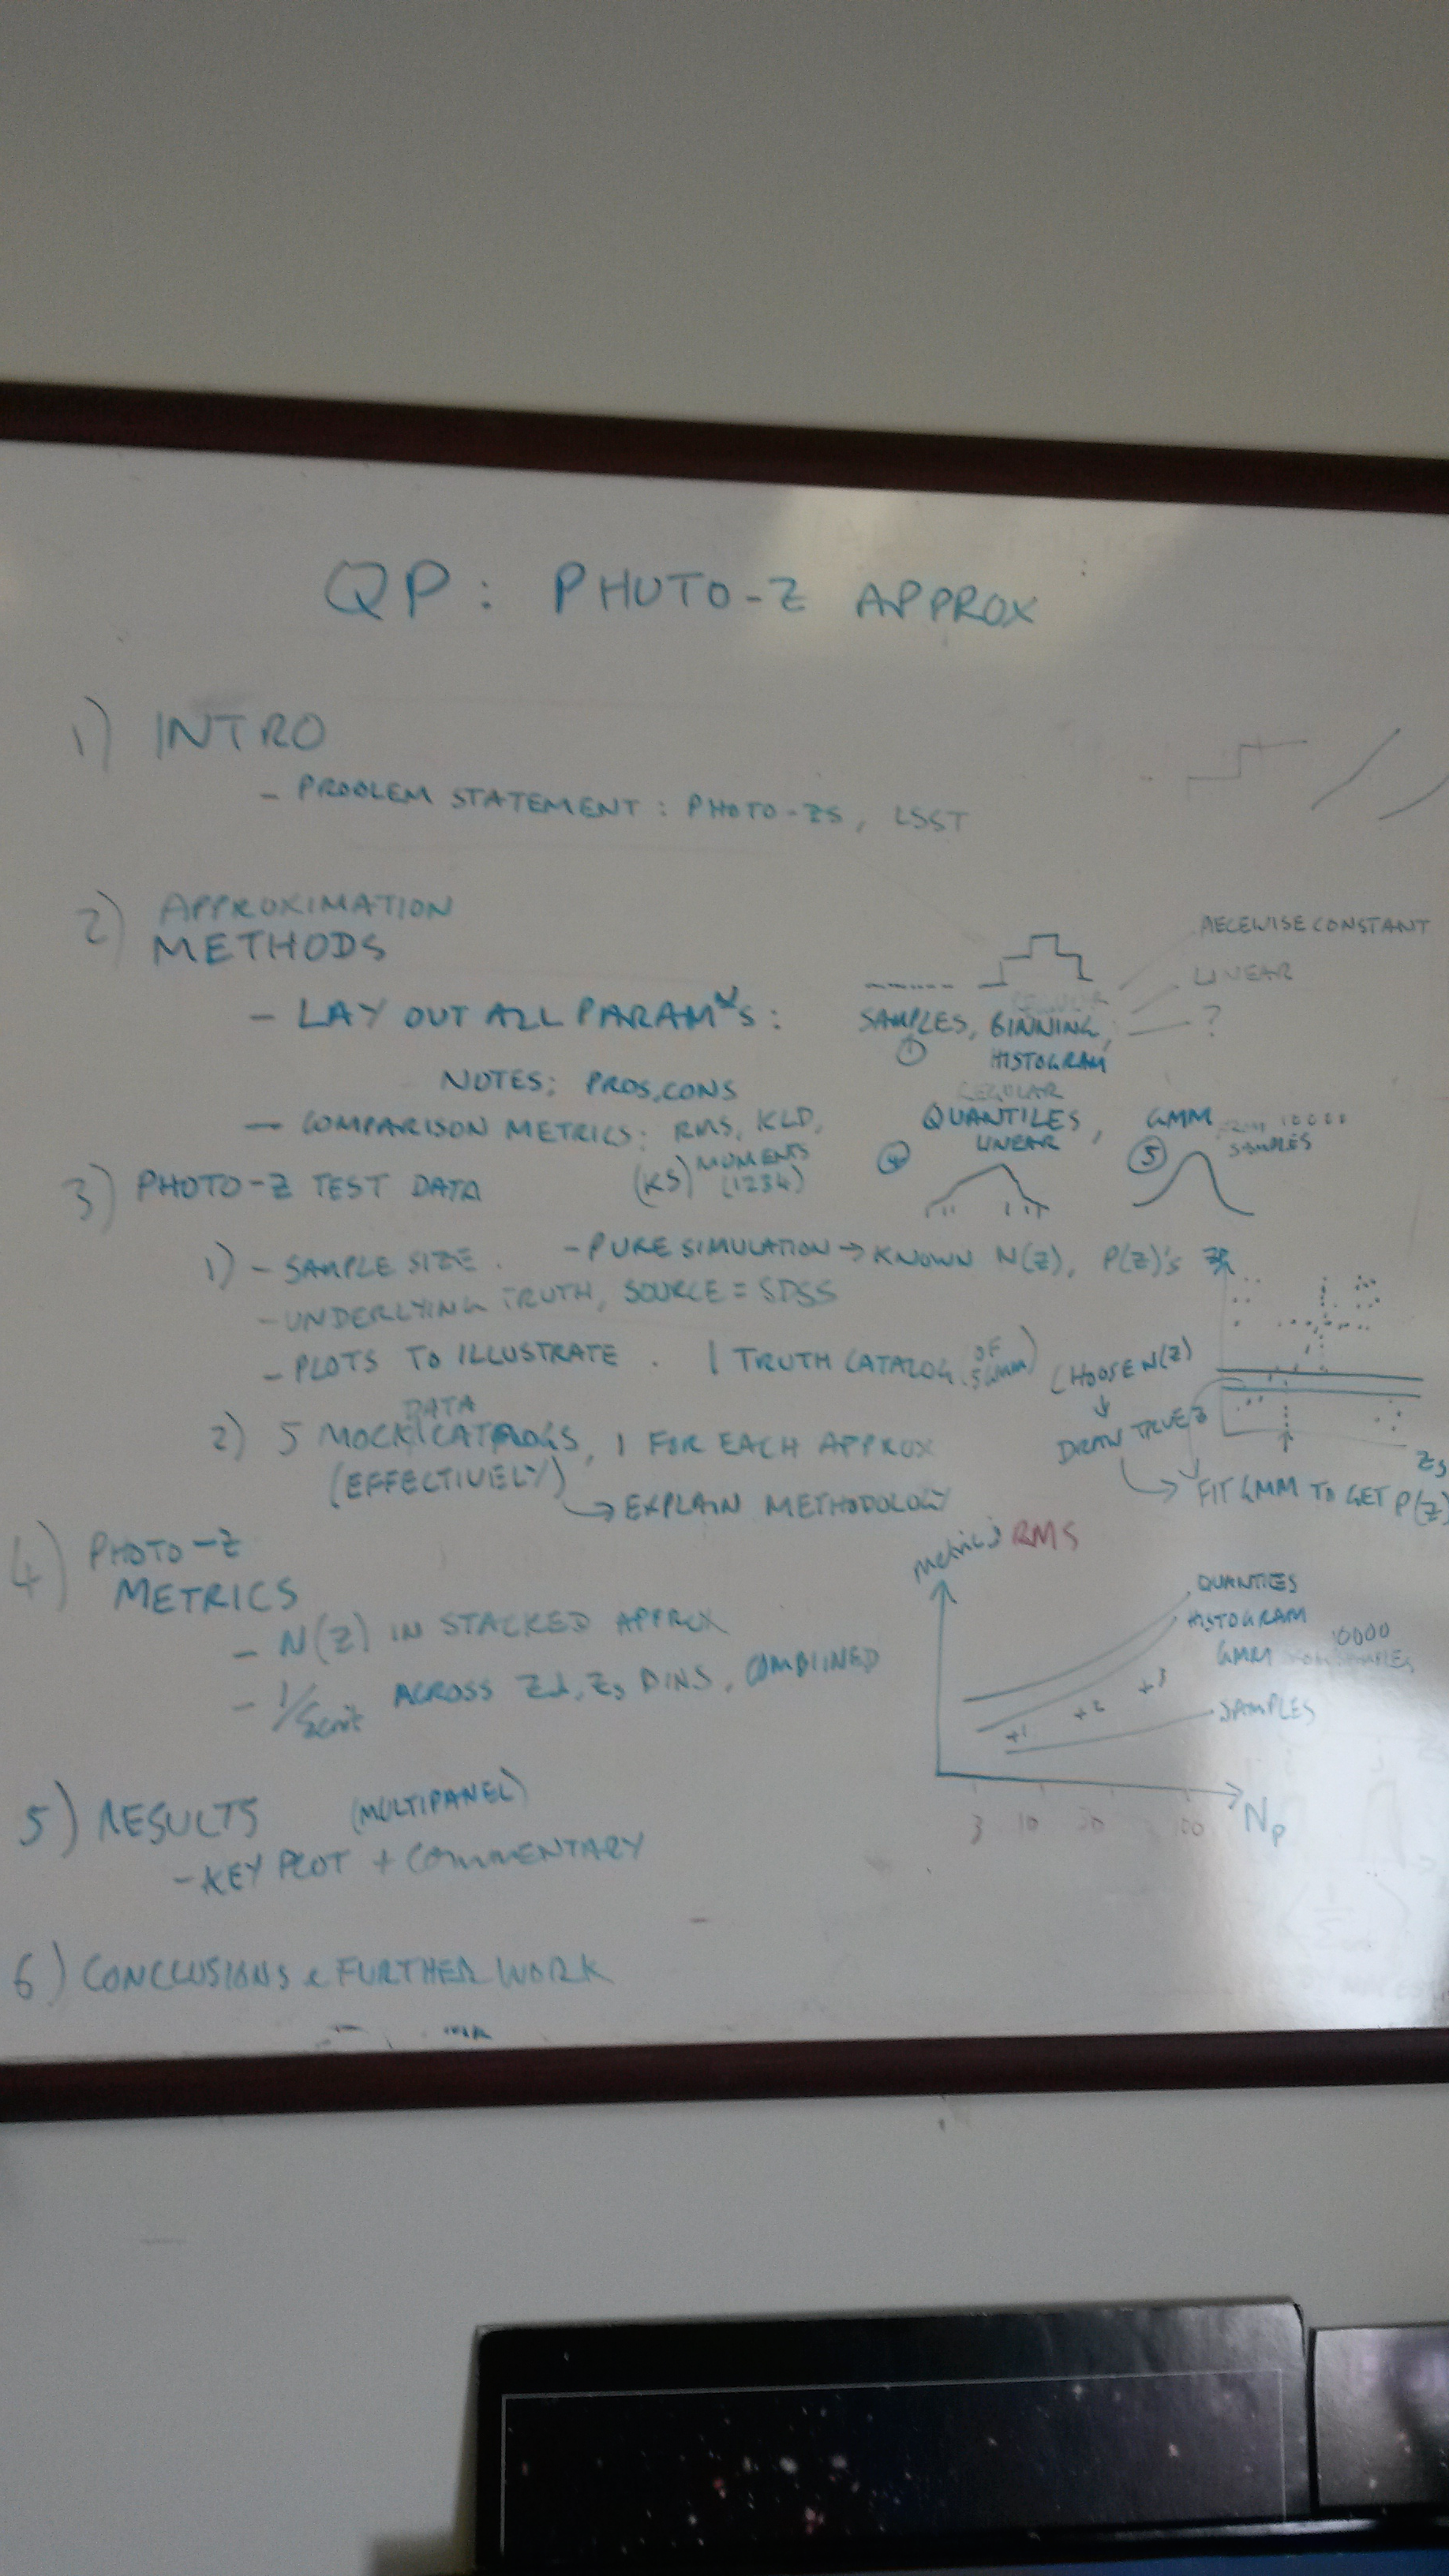
\includegraphics[width=0.75\columnwidth]{outline.png}
%\caption{}. \label{fig:outline}}
%\end{figure}

\section{Introduction}
\label{sec:intro}

%This is a paper and note template for the LSST DESC \citep{Overview,ScienceBook,WhitePaper}.
%You can delete all this tutorial text whenever you like.
%
%You can easily switch between various \LaTeX\xspace styles for internal notes and peer reviewed journals.
%Documents can be compiled using the provided \code{Makefile}.
%The command \code{make} with no arguments compiles \code{main.tex} using the  \code{lsstdescnote.cls} style.
%If you want to upgrade your Note into a journal article, just choose a journal name, between \code{make apj} (ApJ preprint format), \code{make apjl} (which uses the \code{emulateapj} style), \code{make prd}, \code{make prl}, and \code{make mnras}.

Ongoing and upcoming photometric galaxy surveys such as the Large Synoptic Survey Telescope (LSST) will observe tens of billions of galaxies without spectroscopic follow-up to obtain redshifts necessary for studies of cosmology and galaxy evolution.  Such surveys rely on the methods of photometric redshift (photo-$z$) estimation.  Photo-$z$s are subject to a number of systematic errors, some caused by the data analysis procedures and others intrinsic to the data itself.  Due to these issues, the photo-$z$ community favors estimation of redshift probability distributions, or photo-$z$ PDFs, that include information about the potential for such systematic errors for each galaxy in the survey.

Given the tremendous size of the surveys in question, storage of these probability distributions raises a number of nontrivial questions.  Previous treatments of photometric redshifts resulted in each galaxy's catalog entry having one additional floating point number to store, or perhaps a few based on a handful of photo-$z$ codes; how many numbers are necessary to characterize a photo-$z$ PDF to the degree of precision dictated by the survey's science goals?  Photo-$z$ PDF codes do not all produce outputs in the same parametrization; what storage format best preserves the characteristics of a photo-$z$ PDF?

Little attention has been paid to these matters, with a few exceptions.  \citep{carrasco_kind_sparse_2014}

In this work, we outline a method by which a survey team may optimize the choice of parametrization and number of stored parameters for an anticipated catalog of photo-$z$ PDFs.  We also present the publicly available \qp Python package for performing this optimization for an arbitrary survey.  The approach is demonstrated for LSST mock data.

%[Problem statement: photo-zs, LSST]


% ----------------------------------------------------------------------

%\section{Commands}
%\label{sec:commands}

%There are a number of useful \LaTeX\xspace commands predefined in \code{macros.tex}.
%Notice that the section labels are prefixed with \code{sec:} to allow the use of the \verb=\secref= command to reference a section (\ie, \secref{intro}).
%Figures can be referenced with the \verb=\figref= command, which assumes that the figure label is prefixed with \code{fig:}.
%In \figref{example} we show an example figure.
%You'll notice that the actual figure file is found in the \code{figures} directory.
%However, because we have specified this directory in our \verb=\graphicspath= we do not need to explicitly specify the path to the image.
%
%The \code{macros.tex} package also contains some conventional scientific units like \angstrom, \GeV, \Msun, etc. and some editorial tools for highlighting \FIXME{issues}, \CHECK{text to be checked}, \COMMENT{comments}, and \NEW{new additions}.


% ----------------------------------------------------------------------

\section{Methods}
\label{sec:methods}

[Describe possible interpolation schemes used in conversions for both approximations and metrics]

%Similar to the figure before, here we have included a table of data from \code{tables/table.tex}.
%Notice that again we are able to reference \tabref{example} with the \verb=\tabref= command using the \code{tab:} prefix.
%Also notice that we haven't needed to specify the full path to the table because in the \code{Makefile} we include \code{./tables} directory in the \code{\$TEXINPUTS} environment variable.
%
%\input{table}
%
%Equations appear as follows, and can be referred to as, for example, \eqnref{example} -- just as for tables, we use the \verb=\eqnref= command using the \code{eqn:} prefix.
%\begin{equation}
%  \label{eqn:example}
%  \langle f(k) \rangle = \frac{ \sum_{t=0}^{N}f(t,k) }{N}
%\end{equation}

\qp has two main functionalities: converting between parametrizations of photo-$z$ PDFs and computing metrics of parametrizations of photo-$z$ PDFs relative to perfectly accurate representations thereof.

\subsection{Approximation Methods}
\label{sec:approx}

%[Lay out all parametrizations, pros and cons]

\qp is capable of converting a one-dimensional probability distribution between four parametrizations that have been used in the literature as well as one that has not: step functions, samples, grid evaluations, a mixture model, and quantiles.  These parametrizations will be described below in terms of the number $N_{p}$ of parameters $i$.

\COMMENT{I need to hunt down citations for the assertion that these formats have been used before!}

\subsubsection{Regular Binning}
\label{sec:bins}

By far the most common parametrization of photo-$z$ PDFs is that of a piecewise constant step function, also called a histogram binning.  \citep{tanaka_photometric_2017}

\subsubsection{Samples}
\label{sec:samples}

Some surveys store samples of a photo-$z$ PDF.

\subsubsection{Evaluation on a Regular Grid}
\label{sec:grid}

\subsubsection{Mixture Model}
\label{sec:mm}

There is some history of using a mixture model parametrization for photo-$z$ PDFs.  Though mixtures of Gaussian distributions have been used more often, other functions have been investigated as well \citep{carrasco_kind_sparse_2014}.

In this work, we consider only the common Gaussian mixture model, though the \qp framework can accommodate mixtures of all probability distribution functions that have been implemented as \texttt{scipy.stats.rv_continous} objects.

Though the sparse basis representation of \citet{carrasco_kind_sparse_2014} has promising compression properties, we do not consider it in this work for several reasons.  The sparse basis representation of \citet{carrasco_kind_sparse_2014} does not guarantee that the stored parametrization be a probability distribution in a mathematical sense, which we consider a necessary condition both for use of photo-$z$ PDFs in research and for comparison to other methods using the \qp metrics.   The sparse basis representation also assumes that the native format of a photo-$z$ PDF is evaluations on a grid; if this is not true, then the photo-$z$ PDF may undergo additional conversions that introduce loss of information with each approximation.

\COMMENT{I also thought it required extensive computational resources, but it appears to be a lot faster than \qp making quantiles with the same number of parameters -- recall that calculating quantiles generally requires an optimization.  My reasons are pretty weak; if I had more time I'd have \qp employ the \texttt{SparsePz} method as another parametrization, but I don't know when I'll be able to do it!}

\subsubsection{Regular Quantiles}
\label{sec:quantiles}

One parametrization that has not previously been implemented is that of quantiles, which are defined in terms of the cumulative distribution function (CDF)
\begin{align}
  \label{eq:cdf}
  CDF &= \int_{-\infty}^{z}\ p(z)\ dz.
\end{align}
Under the quantile parametrization, an ensemble of photo-$z$ PDFs shares a set of $N$ values $0<q_{1}<q_{2}<\dots<q_{N-1}<q_{N_{p}}<1$.  Each galaxy's catalog entry is the $N_{p}$ values $z_{i}$ satisfying $CDF=q_{i}$.  In our tests, the quantiles obey a regular binning $q_{i}\equiv i\bar{q}$, where $\bar{q}\equiv(N_{p}+1)^{-1}$, but there is no requirement that this be so.

\subsection{Comparison Metrics}
\label{sec:metrics}

%[Lay out all metrics considered, pros and cons]

We use several metrics to quantify how well an approximation of a photo-$z$ PDF reconstructed from a stored format represents the original photo-$z$ PDF before it was compressed.

\COMMENT{\citet{carrasco_kind_sparse_2014} uses histograms and summary statistics of the RMSE distribution.  Should we also do that or is it sufficient to interpret the metrics on $\hat{n}(z)$ in terms of percent error?}

\COMMENT{\citet{carrasco_kind_sparse_2014} and others also consider metrics on point estimators derived from PDFs which I implement for the PZ DC1 paper.  Should I include that in this paper?}

\subsubsection{RMSE}
\label{sec:rms}

The root mean square error (RMSE) is a familiar measure of the difference between two functions.  The

\subsubsection{KLD}
\label{sec:kld}

The Kullback-Leibler divergence quantifies the deviation of one distribution from another, which in our case is the distance to a true distribution $P$ from an approximation thereof $P'$, as in
\begin{align}
  D(P' | P) &= \int_{-\infty}^{\infty}\ \log\left[\frac{P(z)}{P'(z)}\right]\ P(z)\ dz.
\end{align}

%\subsubsection{Moments}
%\label{sec:moments}

%\subsubsection{KS}
%\label{sec:ks}

% ----------------------------------------------------------------------

\section{Photo-z Test Data}
\label{sec:data}

With the expectation that \qp may suggest a different optimal result for different datasets, we apply it to two mock datasets with different data quality properties.  Both datasets were fit using Bayesian Photometric Redshift (BPZ) estimation \citep{benitez_bayesian_2000}, which employs spectral energy distribution (SED) fitting to a template set.  However, the choice of photo-$z$ PDF estimation method is not relevant to this study; so long as the mock photo-$z$ PDFs are of realistic complexity, it does not matter how accurately they describe the probability distribution of galaxy redshifts given their photometric data.  We only seek to optimize the fidelity of the stored photo-$z$ PDF relative to the photo-$z$ PDF output by a representative photo-$z$ PDF fitting code.  (Other work has been done to compare the accuracy of photo-$z$ PDFs produced by different methods; see Schmidt, et al. 2017 (in prep.), \citet{tanaka_photometric_2017}.)

As BPZ is a widely used and well established method, we assume that the photo-$z$ PDFs produced by it are of realistic complexity, meaning they take shapes we expect to see in accurate photo-$z$ PDFs from datasets with similar photometric properties.

\COMMENT{\citet{carrasco_kind_sparse_2014} uses $N_{g}=10^{6}$ galaxies.}

\subsection{LSST+Euclid mocks}
\label{sec:mg}



\subsection{LSST mocks}
\label{sec:ss}

%\subsection{Simulation}
%\label{sec:mock}

%["Observed" $z_{s}$ vs. $z_{p}$ (from Buzzard)]

%\begin{figure}
%%\includegraphics[width=0.9\columnwidth]{}
%\caption{[plot of $z_{s}$ vs. $z_{p}$]\label{fig:observed}}
%\end{figure}

%[Fit $z_{s}$ vs. $z_{p}$ with bivariate GMM]

%\begin{figure}
%%\includegraphics[width=0.9\columnwidth]{}
%\caption{[$z_{s}$ vs. $z_{p}$ contour plot after GMM fit]\label{fig:fit}}
%\end{figure}

%[Specify true $n(z)$]

%\begin{figure}
%%\includegraphics[width=0.9\columnwidth]{}
%\caption{[chosen true $n(z)$]\label{fig:nz}}
%\end{figur}

%\subsection{Catalog generation}
%\label{sec:catalogs}

%[Choose catalog size $N$ and sample $z_{s}$ values from true $n(z)$]

%[Evaluate $N$ "true" $p(z)$s from horizontal cuts in fitted $z_{s}$ vs. $z_{p}$; these are \texttt{qp.catalog} objects comprised of \texttt{qp.PDF} objects defined by original GMM formulae]

%\begin{figure}
%%\includegraphics[width=0.9\columnwidth]{}
%\caption{[Some example $p(z)$s]\label{fig:pzs}}
%\end{figure}

%[Convert into parametrizations as separate catalogs]

% ----------------------------------------------------------------------

\section{Science Metrics}
\label{sec:science}

Though the use of photo-$z$ PDFs could potentially extend to all areas of astronomy in which redshifts are used, photo-$z$ PDFs have thus far been used almost exclusively to estimate the redshift distribution function $n(z)$ necessary for calculating correlation functions used in many cosmological probes.  The most common way to estimaate the redshift distribution function is to "stack" the photo-$z$ PDFs.

\subsection{$\hat{n}(z)$}
\label{sec:nz}

Though we do not recommend this approach to estimating the redshift distribution (see Malz, et al. (in prep.) for a mathematically motivated alternative), we also calculate the metrics of Sec. \ref{sec:metrics} on the stacked estimator
\begin{align}
  \label{eq:nz}
  \hat{n}(z) &= \frac{1}{N_{g}}\sum_{j=1}^{N_{g}}
 p_{j}(z)
\end{align}
of the redshift distribution function.

%\subsection{$\Sigma_{crit}^{-1}$}
%\label{sec:sigma}

%\citet{dark_energy_survey_collaboration_redshift_2016}

%\begin{align}
%\Sigma_{crit}^{-1} &= \frac{4\pi G}{c}\frac{D_{ls}D_{l}}{D_{s}}
%\label{eq:sigma}
%\end{align}

%\begin{align}
%\left\langle\Sigma_{crit}^{-1}\right\rangle(z_{lens}) &= \sum_{i=1}^{N}p(z_{source, i})\Sigma_{crit}^{-1}(z_{lens}, z_{source, i})
%\label{eq:meansigma}
%\end{align}

% ---------------------------------------------------------------------

\section{Results}
\label{sec:results}

%\figref{example} shows an example figure, referred to with the \verb=\figref= command and the \code{fig:} prefix.
%
%\begin{figure}
%\includegraphics[width=0.9\columnwidth]{example.png}
%\caption{An example figure: the LSST DESC logo, copied from \code{.logos/desc-logo.png} into \code{figures/example.png}. \label{fig:example}}
%\end{figure}

\subsection{Individual photo-$z$ PDFs}
\label{sec:individual}

Parametrizations are compared on the basis of the distributions of the metrics of Sec. \ref{sec:metrics} calculated over the ensemble.

\begin{figure}
%\includegraphics[width=0.9\columnwidth]{}
  \caption{[number of stored floats $N$ vs. metric value, one curve per approximation method, one panel per combination of metric (horizontal) and $N$ (vertical)]
  \label{fig:individual}}
\end{figure}

\subsection{Stacked $\hat{n}(z)$ estimator}
\label{sec:stacked}

Parametrizations are also compared by the accuracy of their stacked redshift distribution estimator $\hat{n}(z)$ relative to that of the photo-$z$ PDFs in their original format.

\begin{figure}
%\includegraphics[width=0.9\columnwidth]{}
  \caption{[number of stored floats $N$ vs. metric value, one curve per approximation method, one panel per combination of metric (horizontal) and $N$ (vertical)]
  \label{fig:stacked}}
\end{figure}

% ----------------------------------------------------------------------

%\section{Discussion}
%\label{sec:discussion}
%
%If you are planning on committing your paper to GitHub, it's a good idea to write your tex as one sentence per line.
%This allows for an easier \code{diff} of changes.
%It also makes sense to think of latex as \emph{code}, and sentences as logical statements, occupying one line each.
%Each line must ``compile'' in the mind of the reader.


% ----------------------------------------------------------------------

\section{Conclusions \& Future Directions}
\label{sec:conclusions}

%Here's a summary of what we just reported.
%
%We can draw the following well-organized and neatly-formatted conclusions:
%\begin{itemize}
%  \item This is important.
%  \item We can measure some number with some precision.
%  \item This has some implications.
%\end{itemize}
%
%Here are some parting thoughts.

% ----------------------------------------------------------------------

This work addresses the tradeoff between the accuracy of stored photo-$z$ PDFs and the footprint of the data needed to encode the photo-$z$ PDFs.  It does not address the computational resources necessary to perform the storage operation nor to unpack the stored information into the form necessary for science computations.

Further applications of \qp functionality for manipulations of photo-$z$ PDFs is demonstrated in the LSST-DESC PZ DC1 paper (in prep.).

\subsection*{Acknowledgments}

%Here is where you should add your specific acknowledgments, remembering that some standard thanks will be added via the \code{acknowledgments.tex} and \code{contributions.tex} files.

We thank Melissa Graham and Sam Schmidt for providing the mock datasets.  This work was incubated at the 2016 LSST-DESC Hack Week.

\input{acknowledgments}

Author contributions are listed below. \\
A.I.~Malz: Initiated project, led development work. \\
P.J.~Marshall: Advised on statistics, and project design and management. \\
S.J.~Schmidt: Provided the Optical dataset. \\
M.~Graham: Provided the Optical+IR dataset. \\
J.~DeRose: Contributed to the production of the Optical dataset. \\
R.~Wechsler: Contributed to the production of the Optical dataset. \\


%{\it Facilities:} \facility{LSST}

% Include both collaboration papers and external citations:
\bibliography{lsstdesc,main}
%\bibliography{qp}

\end{document}
% ======================================================================
%
